%% =====================================================================
%% Paper (doble columna): Transferibilidad de un modelo geoespacial de
%% localizacion a otros servicios urbanos en Arequipa Metropolitana
%% Compilar con:  tectonic main.tex      (o pdflatex dos veces)
%% Las referencias están escritas a mano en estilo APA 7 (sección final).
%% =====================================================================
\documentclass[10pt,letterpaper,twocolumn]{article}

\usepackage[utf8]{inputenc}
\usepackage[T1]{fontenc}
\usepackage{mathptmx}
\usepackage[spanish,es-nodecimaldot,es-tabla]{babel}
\usepackage[top=0.8in,bottom=0.85in,left=0.75in,right=0.75in,columnsep=0.25in]{geometry}
\usepackage{amsmath}
\usepackage{booktabs}
\usepackage{graphicx}
\usepackage{caption}
\usepackage[hyphens]{url}
\usepackage[hidelinks,colorlinks=true,linkcolor=black,citecolor=black,urlcolor=blue]{hyperref}
\usepackage[round,authoryear]{natbib}
\usepackage{microtype}
\usepackage{array}
\usepackage{balance}

\setlength{\parindent}{0.9em}
\setlength{\parskip}{0pt}
\setlength{\emergencystretch}{1.5em}
\Urlmuskip=0mu plus 2mu
\captionsetup{font=small,labelfont=bf,labelsep=period,skip=4pt}
\setlength{\bibsep}{2pt}
\bibpunct[, ]{(}{)}{;}{a}{}{,}
\setlength{\textfloatsep}{8pt plus 2pt minus 2pt}
\setlength{\floatsep}{8pt plus 2pt minus 2pt}
\setlength{\intextsep}{8pt plus 2pt minus 2pt}

\begin{document}

\twocolumn[{%
\begin{center}
{\LARGE\bfseries \textquestiondown{}Se transfiere un modelo geoespacial de localización a otros servicios urbanos? Evidencia de ocho usos en Arequipa Metropolitana}\\[1.1em]
{\large Fernando Gabriel Casapía Loayza\,$^{1}$ \quad Paolo Marcelo Rivera Salas\,$^{1}$ \quad Karina Rosas Paredes\,$^{1}$}\\[0.5em]
{\small $^{1}$Escuela Profesional de Ingeniería de Sistemas, Universidad Católica de Santa María, Arequipa, Perú}\\[0.3em]
{\small \texttt{fernando.casapia@estudiante.ucsm.edu.pe} \quad \texttt{paolo.rivera@estudiante.ucsm.edu.pe} \quad \texttt{kparedes@ucsm.edu.pe}}\\[0.3em]
{\footnotesize ORCID: 0009-0001-3899-1474 \quad 0009-0004-2718-3780 \quad 0000-0003-4650-7432}
\end{center}
\vspace{0.4em}
\begin{center}
\begin{minipage}{0.94\textwidth}
\small
\noindent\textbf{Resumen.}
Las ciudades necesitan decidir dónde ubicar servicios como farmacias, bancos, colegios o grifos, pero los modelos que ayudan a hacerlo se construyen para un solo servicio, y no se sabe si lo que aprenden sirve para otro, lo que obliga a reunir datos nuevos cada vez. Esta investigación tuvo como objetivo evaluar si un mismo modelo de aprendizaje automático, creado para ubicar minimarkets, puede aplicarse a otros siete usos en Arequipa Metropolitana: farmacias, grifos, bancos y cajeros, colegios, restaurantes, clínicas y hospitales, y mercados. Se dividió la ciudad en 3\,717 hexágonos de unos 0,11\,km$^2$, se usaron datos públicos del Censo 2017 y de OpenStreetMap, y se midió qué tan bien el modelo distingue los hexágonos donde ya existe cada servicio de los que no (0,5 equivale al azar y 1 a un acierto perfecto), siempre sobre zonas de la ciudad que el modelo no vio al aprender. El modelo obtuvo entre 0,85 y 0,93 sobre toda la ciudad y entre 0,67 y 0,86 en las zonas con población suficiente para sostener un negocio, y fue mejor que una regla simple basada solo en la población en cinco de los ocho usos. Además, un modelo aprendido con un servicio acertó, en promedio, 0,88 al aplicarse a los demás, y el modelo hecho a medida de cada servicio fue el mejor solo en tres de ocho, aunque los servicios casi nunca ocupan los mismos hexágonos. Se concluye que la ubicación de los servicios sigue en gran parte un mismo patrón urbano, el de las zonas más pobladas y activas, por lo que un modelo entrenado con un servicio puede dar una primera orientación para otro; las diferencias propias de cada servicio son menores y aparecen en la red de calles para los grifos y en la cercanía a otros servicios para bancos, restaurantes y clínicas.

\smallskip
\noindent\textit{Palabras clave:} localización de servicios, transferibilidad, analítica geoespacial

\medskip
\noindent\textbf{Abstract.}
Cities need to decide where to place services such as pharmacies, banks, schools, or gas stations, but the models that support these decisions are built for a single service, and it is unknown whether what they learn applies to another, which forces new data to be gathered each time. This research aimed to assess whether a single machine-learning model, created to locate minimarkets, can be applied to seven other land uses in Metropolitan Arequipa: pharmacies, gas stations, banks and ATMs, schools, restaurants, clinics and hospitals, and markets. The city was divided into 3,717 hexagons of about 0.11\,km$^2$, public data from the 2017 Census and OpenStreetMap were used, and the model's ability to tell the hexagons where each service exists from those where it does not was measured (0.5 equals chance and 1 a perfect score), always on areas of the city the model had not seen while learning. The model scored between 0.85 and 0.93 across the whole city and between 0.67 and 0.86 in areas with enough population to sustain a business, and it outperformed a simple population-only rule in five of the eight uses. In addition, a model learned with one service scored 0.88 on average when applied to the others, and the model tailored to each service was the best in only three of eight, even though the services almost never occupy the same hexagons. It is concluded that service location largely follows a single urban pattern, that of the most populated and active areas, so a model trained on one service can offer a first guide for another; the differences specific to each service are smaller and appear in the street network for gas stations and in proximity to other services for banks, restaurants, and clinics.

\smallskip
\noindent\textit{Keywords:} service location, transferability, geospatial analytics
\end{minipage}
\end{center}
\vspace{0.8em}
}]

%% ---------------------------------------------------------------------
\section{Introducción}

Decidir dónde ubicar un establecimiento es un problema clásico de la geografía del comercio \citep{huff1964,christaller1966}. Con la disponibilidad de datos geoespaciales, el problema se ha trasladado al aprendizaje automático: modelos entrenados con el entorno urbano predicen la popularidad de una tienda \citep{karamshuk2013}, seleccionan locales de cadenas comerciales \citep{lu2024,zhao2025} o explican el efecto del entorno sobre la ubicación minorista \citep{zhang2025}. Casi todos esos trabajos se construyen para un solo uso del suelo y con insumos privados, como series de ventas \citep{lu2024,hu2025} o señalización de telefonía móvil \citep{zou2024}.

Esa práctica deja sin responder una pregunta con consecuencias para las ciudades con pocos datos: si el perfil de localización que aprende un modelo para un uso, por ejemplo el minimarket, sirve también para otros usos, como una farmacia, un banco o un colegio. Si se transfiere, un solo modelo entrenado donde hay datos podría orientar decisiones donde no los hay. Si no se transfiere, cada servicio exigiría su propio modelo y sus propios datos. La literatura revisada no contrasta ambas posibilidades de forma explícita, ni lo hace con la validación espacial que exige la autocorrelación del territorio \citep{ploton2020,roberts2017,meyer2021}.

Este trabajo toma el modelo desarrollado para localizar minimarkets independientes en Arequipa Metropolitana \citep{casapia2026} y lo aplica, sin modificarlo, a siete usos adicionales. Se plantean tres preguntas: (i) \textquestiondown{}con qué capacidad discrimina el mismo modelo la localización de cada uso y mejora a criterios simples de demanda? (ii) \textquestiondown{}qué determina la localización de cada uso? (iii) \textquestiondown{}hasta qué punto un modelo entrenado con un uso predice la localización de los demás? Las contribuciones son una evaluación de ocho usos con el mismo diseño de validación, una matriz de transferencia entre ellos con control de fuga de información y un análisis de qué parte de la señal es común y qué parte es propia de cada servicio.

%% ---------------------------------------------------------------------
\section{Materiales y métodos}

\subsection{Unidad de análisis y datos}

El área de estudio comprende los diecisiete distritos de Arequipa Metropolitana. Se discretizó en 3\,717 celdas hexagonales H3 de resolución~9 \citep{brodsky2018,kmoch2022}, de $\approx$0,11\,km$^2$ cada una, y se reconoce la sensibilidad de los resultados a esta zonificación \citep{openshaw1984}. La demanda poblacional proviene del Censo 2017 (1\,018\,031 habitantes en 21\,705 manzanas; \citealp{inei2018}), transferida a la celda por ponderación areal. Las ubicaciones de los servicios y la red vial proceden de OpenStreetMap, con licencia ODbL. Se construyeron 37 predictores en cuatro familias: demanda poblacional en anillos de vecindad, morfología vial, puntos de interés (POI) por categoría y competencia comercial observada. El diseño completo de los predictores se describe en \citet{casapia2026}.

\subsection{Objetivos}

Para cada uno de los siete servicios la variable objetivo es binaria: la celda contiene al menos un establecimiento mapeado en OpenStreetMap. Como referencia se incluye el minimarket, definido como las celdas con una tienda de la cadena de descuento duro según su localizador público en 2026, que es el objetivo del estudio previo. La Tabla~\ref{tab:objetivos} resume los ocho objetivos.

\begin{table}[t]
\centering
\caption{Usos evaluados, establecimientos mapeados y celdas con presencia.}
\label{tab:objetivos}
\footnotesize
\setlength{\tabcolsep}{3pt}
\begin{tabular}{>{\raggedright\arraybackslash}p{2.5cm}rrr}
\toprule
Uso & Establec. & Celdas & Tasa base \\
\midrule
Farmacias & 140 & 72 & 1,9\,\% \\
Grifos & 152 & 138 & 3,7\,\% \\
Bancos y cajeros & 154 & 67 & 1,8\,\% \\
Colegios & 992 & 579 & 15,6\,\% \\
Restaurantes & 643 & 218 & 5,9\,\% \\
Clínicas y hospitales & 123 & 95 & 2,6\,\% \\
Mercados & 94 & 69 & 1,9\,\% \\
Minimarkets (referencia) & 127 & 122 & 3,3\,\% \\
\bottomrule
\end{tabular}
\end{table}

\subsection{Control de fuga de información}

Los predictores incluyen conteos de POI por categoría, de modo que un modelo podría predecir un servicio a partir de su propio conteo en la celda o en su vecindad. Para cada uso se retiran los conteos de su propia categoría y el total de POI de la vecindad, que la contiene, lo que deja 34 predictores (36 para el minimarket). Para la transferencia entre usos se emplea además un perfil estructural de 18 predictores sin ningún conteo de POI (demanda poblacional, morfología vial y competencia), de modo que el modelo de un uso no pueda filtrar información de la categoría de otro. Como control adicional frente a un sesgo común de cobertura, ya que etiquetas y competencia provienen ambas de OpenStreetMap, se repite el análisis con un perfil demográfico-vial de 15 predictores, sin POI ni competencia.

\subsection{Modelos y validación}

Se usó la configuración del estudio previo: regresión logística con regularización L2 ($C=0{,}5$), Random Forest \citep{breiman2001} con 800 árboles y XGBoost \citep{chen2016} con 400 árboles y profundidad 3, ambos con ponderación de clases \citep{he2009}, y un ensamble por promedio de rangos percentiles. La validación fue una validación cruzada espacial de cinco pliegues agrupada por el hexágono padre de resolución~6 (52 bloques). Random Forest y XGBoost se repitieron con cinco semillas (100 a 104) y se reporta la media y la desviación estándar.

Se calcularon el ROC-AUC, el PR-AUC y el lift en el decil superior sobre las 3\,717 celdas, y el ROC-AUC restringido a las 1\,341 celdas \textit{viables}, con al menos 1\,500 habitantes alcanzables en su anillo de vecindad, que son las que un planificador consideraría. Como líneas base se usaron dos criterios univariados: la densidad poblacional y la población alcanzable.

\subsection{Protocolo de transferencia}

Para cada par de usos $(A,B)$ se tomó la puntuación fuera de muestra del ensamble entrenado con el uso $A$ y perfil estructural, y se midió su ROC-AUC contra las celdas positivas del uso $B$. Al usar puntuaciones fuera de muestra, la evaluación no reutiliza las etiquetas de $A$ en las celdas de entrenamiento. La diagonal de la matriz corresponde al propio uso. Se calculó además el índice de Jaccard entre los conjuntos de celdas positivas de cada par.

%% ---------------------------------------------------------------------
\section{Resultados}

\subsection{Capacidad discriminativa por uso}

La Tabla~\ref{tab:res} presenta el desempeño del ensamble. En las 3\,717 celdas el ROC-AUC va de 0,854 (mercados) a 0,926 (colegios), pero la cifra global se infla porque 2\,376 celdas no son viables y resultan negativos fáciles de descartar. En las celdas viables, que son las que ordena un planificador, el ROC-AUC baja a un rango de 0,666 a 0,857. El lift en el decil superior fue de 4,6 a 6,9 veces la tasa base.

\begin{table*}[t]
\centering
\caption{Desempeño del ensamble por uso (validación cruzada espacial, media $\pm$ DE de cinco semillas) frente al mejor criterio univariado en celdas viables.}
\label{tab:res}
\small
\begin{tabular}{lcccccc}
\toprule
Uso & ROC (3\,717) & PR & Lift@10\,\% & ROC viables & Mejor base & Diferencia \\
\midrule
Restaurantes & $0{,}921\pm0{,}001$ & 0,538 & 6,64 & $0{,}857\pm0{,}001$ & 0,688 & $+0{,}168$ \\
Bancos y cajeros & $0{,}896\pm0{,}004$ & 0,259 & 6,89 & $0{,}821\pm0{,}002$ & 0,695 & $+0{,}127$ \\
Farmacias & $0{,}904\pm0{,}001$ & 0,318 & 6,91 & $0{,}822\pm0{,}002$ & 0,730 & $+0{,}092$ \\
Grifos & $0{,}873\pm0{,}001$ & 0,173 & 4,74 & $0{,}745\pm0{,}001$ & 0,671 & $+0{,}074$ \\
Colegios & $0{,}926\pm0{,}000$ & 0,662 & 4,57 & $0{,}781\pm0{,}001$ & 0,762 & $+0{,}019$ \\
Minimarkets (ref.) & $0{,}917\pm0{,}000$ & 0,257 & 6,26 & $0{,}767\pm0{,}001$ & 0,785 & $-0{,}018$ \\
Mercados & $0{,}854\pm0{,}002$ & 0,084 & 5,27 & $0{,}666\pm0{,}004$ & 0,696 & $-0{,}030$ \\
Clínicas y hospitales & $0{,}873\pm0{,}001$ & 0,126 & 5,13 & $0{,}682\pm0{,}001$ & 0,723 & $-0{,}041$ \\
\bottomrule
\end{tabular}
\end{table*}

El ensamble supera al mejor criterio univariado en cinco de los ocho usos, con ventajas de 0,02 a 0,17 en el ROC-AUC de las celdas viables (Figura~\ref{fig:base}). En clínicas, mercados y minimarkets queda por debajo: allí la demanda por sí sola ordena las celdas tan bien como el modelo, o mejor. Las desviaciones entre semillas son menores que 0,005, por lo que reflejan la aleatoriedad del modelo y no la incertidumbre del muestreo de celdas; no se contrastó la significancia de las diferencias.

\begin{figure}[t]
\centering
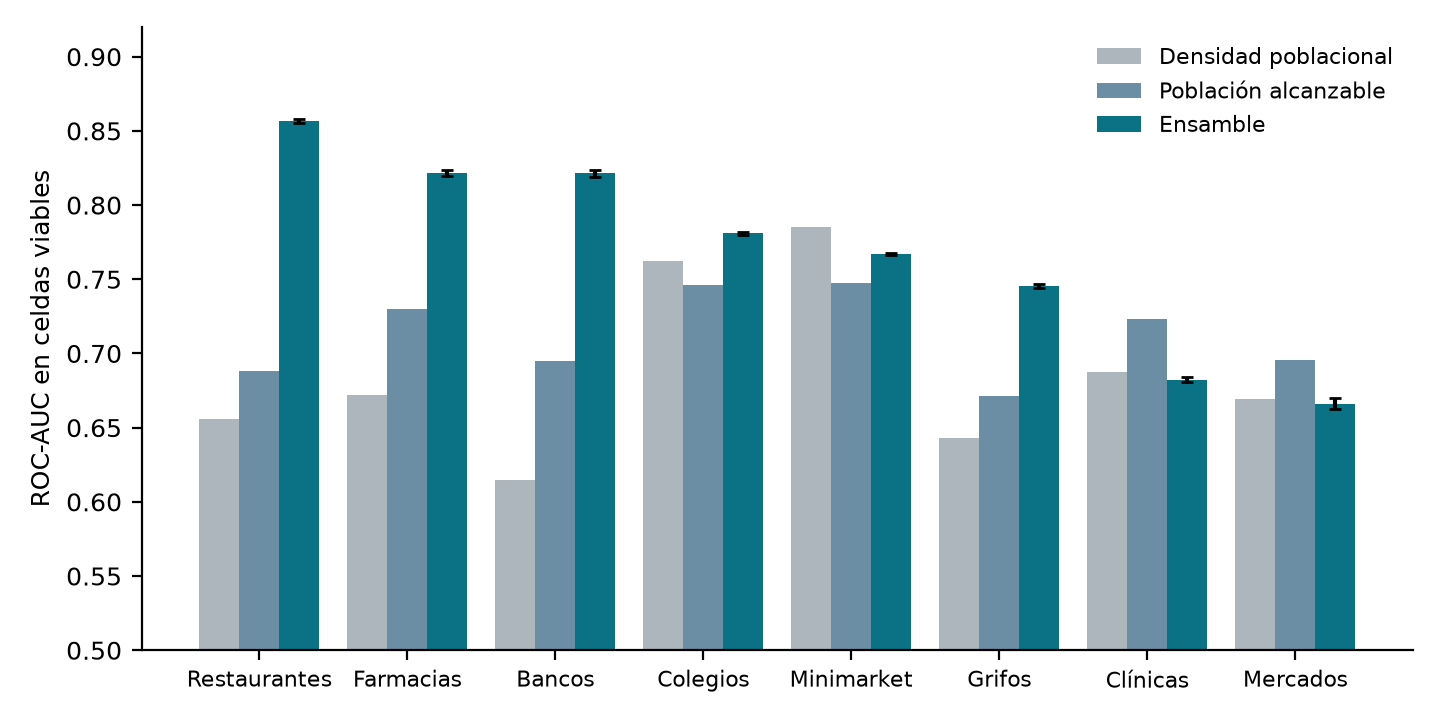
\includegraphics[width=\linewidth]{figuras/fig_baselines.png}
\caption{ROC-AUC en celdas viables del ensamble y de los dos criterios univariados, por uso. Las barras de error son la desviación estándar de cinco semillas. Fuente: elaboración propia.}
\label{fig:base}
\end{figure}

\subsection{Qué determina la localización de cada uso}

La demanda poblacional es la familia dominante en casi todos los usos (Figura~\ref{fig:fam}), pero su peso varía: representa el 69\,\% de la importancia en colegios y el 64\,\% en el minimarket, y baja al 37\,\% en bancos y cajeros. Los grifos son la excepción: su localización depende sobre todo de la red vial, con un 40\,\% de la importancia en la morfología vial y las variables de vía principal entre las tres más importantes. Bancos y farmacias son los usos donde más pesan los POI (37\,\% y 32\,\%), lo que indica aglomeración con otros servicios. Sin ningún POI, el perfil estructural discrimina casi igual o mejor en celdas viables en farmacias, grifos, mercados, colegios y minimarkets, y peor en bancos ($-0{,}046$), restaurantes ($-0{,}019$) y clínicas ($-0{,}036$; Tabla~\ref{tab:conj}). Es decir, solo en esos tres usos los demás servicios aportan información sobre dónde ubicarse.

\begin{figure}[t]
\centering
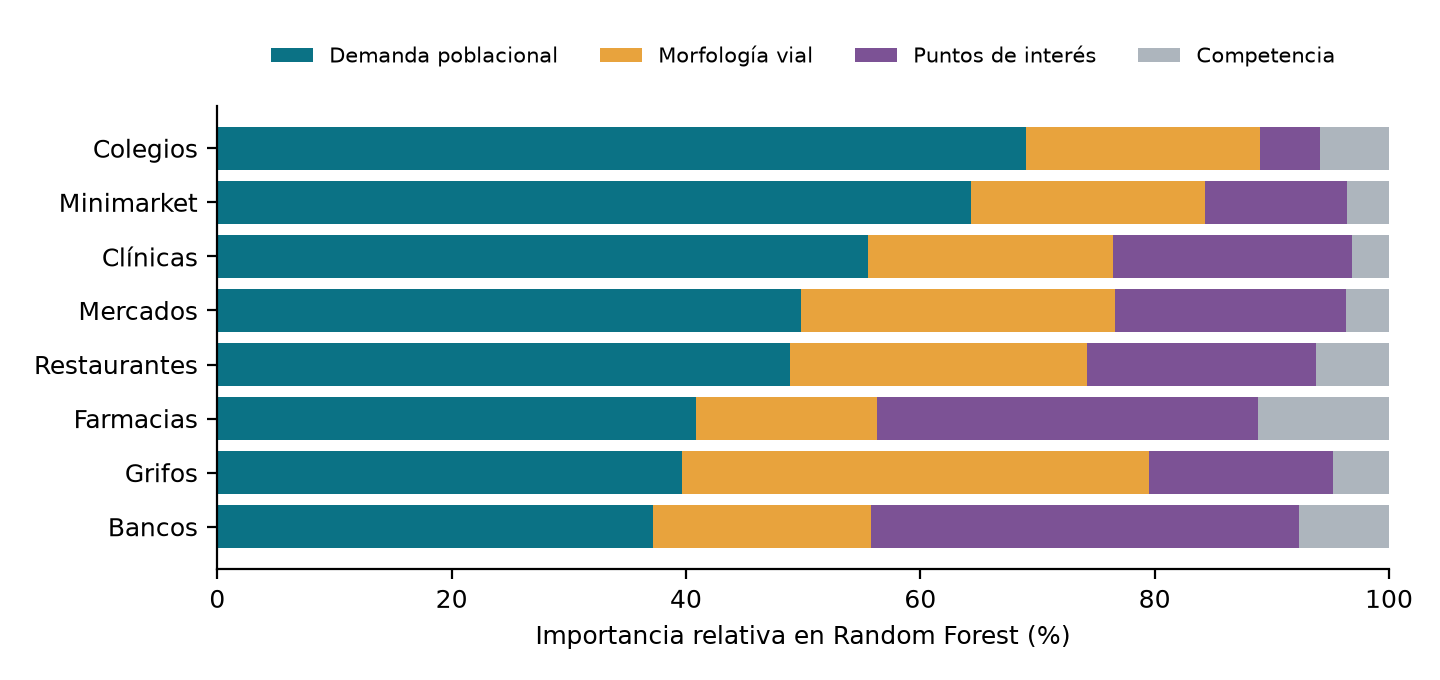
\includegraphics[width=\linewidth]{figuras/fig_familias.png}
\caption{Importancia relativa de cada familia de predictores en Random Forest, por uso. Fuente: elaboración propia.}
\label{fig:fam}
\end{figure}

\begin{table}[t]
\centering
\caption{ROC-AUC del ensamble en celdas viables según el conjunto de predictores.}
\label{tab:conj}
\footnotesize
\setlength{\tabcolsep}{3pt}
\begin{tabular}{>{\raggedright\arraybackslash}p{2.3cm}ccc}
\toprule
Uso & Completo & Estructural & Demog.-vial \\
\midrule
Farmacias & 0,822 & 0,838 & 0,738 \\
Grifos & 0,745 & 0,798 & 0,799 \\
Bancos y cajeros & 0,821 & 0,775 & 0,745 \\
Colegios & 0,781 & 0,776 & 0,773 \\
Restaurantes & 0,857 & 0,838 & 0,774 \\
Clínicas y hosp. & 0,682 & 0,646 & 0,637 \\
Mercados & 0,666 & 0,719 & 0,683 \\
Minimarkets & 0,767 & 0,793 & 0,801 \\
\bottomrule
\end{tabular}
\end{table}

\subsection{Transferencia entre usos}

La Figura~\ref{fig:transfer} muestra la matriz de transferencia. El modelo entrenado con un uso predice bien la localización de los demás: el ROC-AUC fuera de la diagonal tiene una media de 0,884 en todas las celdas (rango 0,814 a 0,959) y de 0,748 en las celdas viables (rango 0,630 a 0,921), frente a medias de 0,900 y 0,773 en la diagonal. El modelo propio fue el mejor en solo tres de los ocho usos en todas las celdas y en dos de ocho en celdas viables. La diferencia entre el modelo propio y el mejor modelo ajeno fue negativa en cinco usos, y en celdas viables llegó a $-0{,}145$ en bancos, $-0{,}107$ en clínicas y $-0{,}067$ en mercados: el modelo de grifos predice mejor la localización de los bancos (0,921) que el propio modelo de bancos (0,775). Los modelos que mejor se exportan son los de grifos y restaurantes (ROC-AUC medio de 0,908 y 0,910 en todas las celdas), y los que peor, en celdas viables, los de clínicas (0,716) y minimarkets (0,690).

\begin{figure*}[t]
\centering
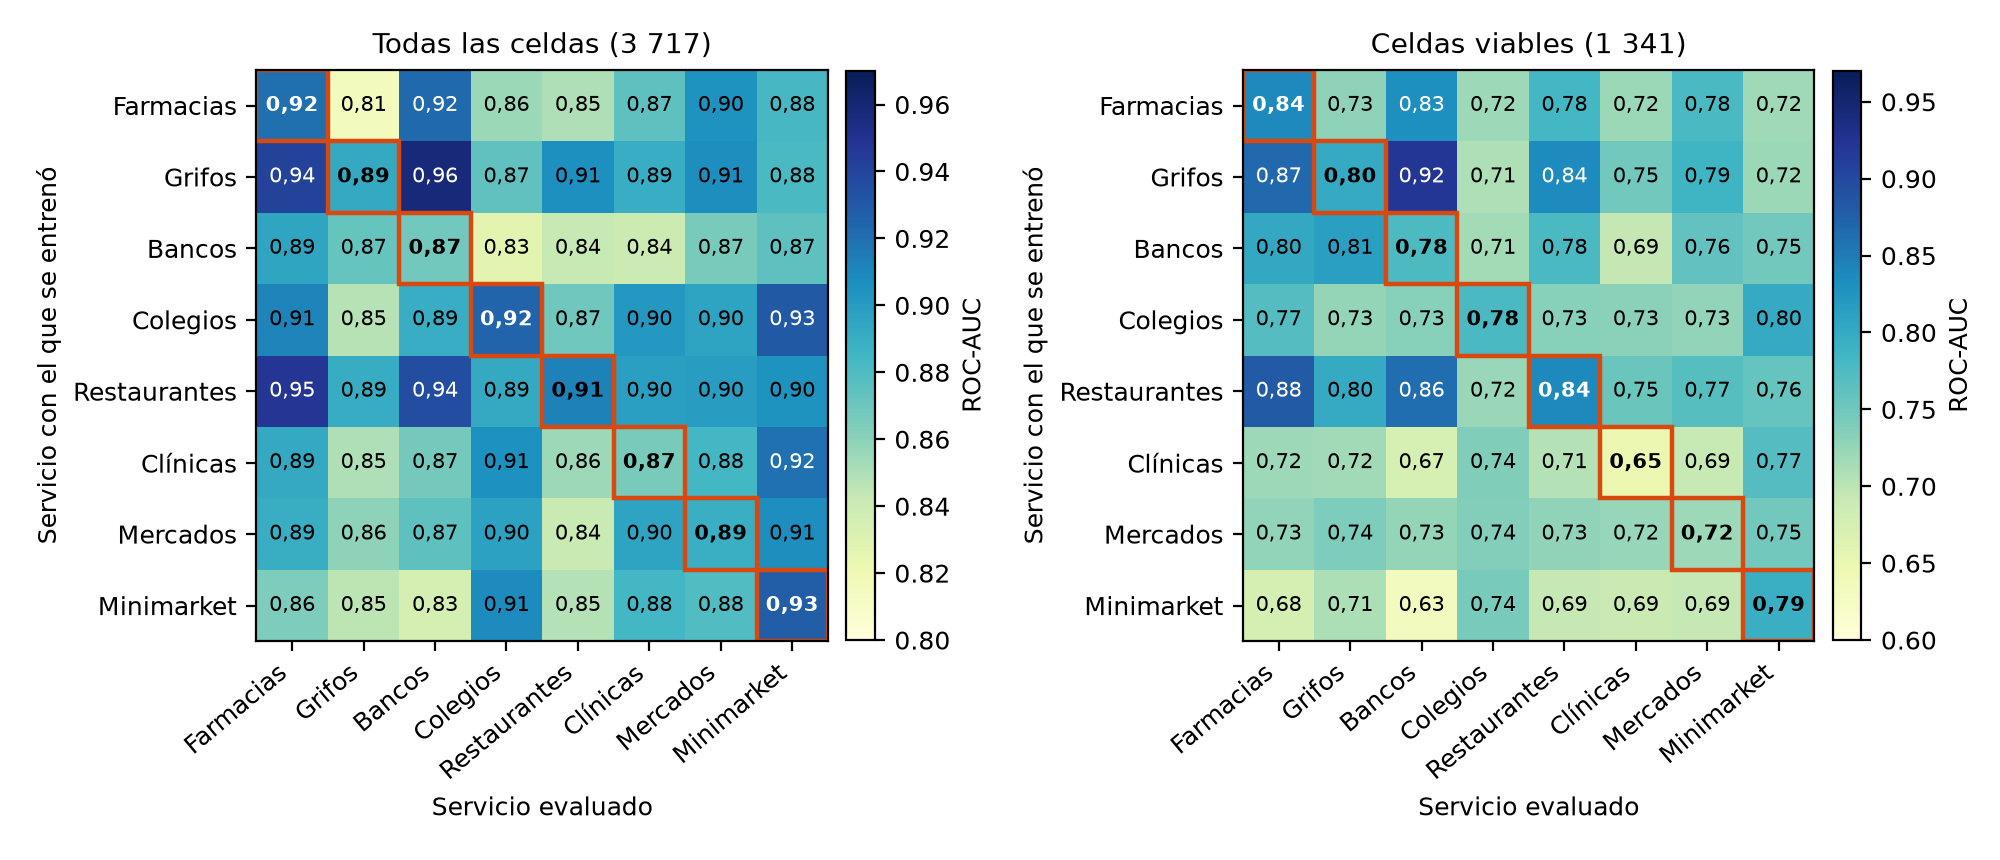
\includegraphics[width=0.92\textwidth]{figuras/fig_transferencia.png}
\caption{Matriz de transferencia: ROC-AUC de la puntuación fuera de muestra del ensamble entrenado con el uso de la fila (perfil estructural) al evaluarlo sobre el uso de la columna. La diagonal (recuadro naranja) es el propio uso. Fuente: elaboración propia.}
\label{fig:transfer}
\end{figure*}

La transferencia es alta aunque los servicios casi no comparten celdas: el índice de Jaccard entre pares de usos tiene una media de 0,13 y un máximo de 0,29 (farmacias y bancos), seguido de 0,23 (farmacias y restaurantes). Es decir, el modelo no está reconociendo las mismas celdas, sino el mismo gradiente de intensidad urbana en el que se sitúan todas.

\subsection{Robustez}

Al retirar los predictores de competencia, que como las etiquetas provienen de OpenStreetMap, el patrón se mantiene: el ROC-AUC fuera de la diagonal tiene una media de 0,880 en todas las celdas y de 0,727 en las viables, y el modelo propio sigue siendo el mejor en tres de los ocho usos en ambos casos. La transferencia, por tanto, no depende del esfuerzo de mapeo que comparten las etiquetas y esa familia de predictores (Tabla~\ref{tab:conj}). El control tiene un costo en farmacias, cuyo ROC-AUC en celdas viables baja de 0,838 a 0,738 sin competencia, lo que sugiere que parte de su localización se asocia a la presencia de otros comercios.

%% ---------------------------------------------------------------------
\section{Discusión}

\textbf{Un gradiente urbano compartido.} Los resultados apuntan a que gran parte de la capacidad de un modelo de localización proviene de un factor común: la intensidad de la actividad urbana, en la que se sitúan todos los servicios. Eso explica que el modelo propio no sea mejor que el ajeno en la mayoría de los usos y que predicciones con un perfil sin POI funcionen casi igual que el modelo completo. Para quien planifica con pocos datos, es una buena noticia práctica: un modelo entrenado en un uso con datos disponibles ofrece una primera aproximación razonable para otro (ROC-AUC medio de 0,75 en celdas viables).

\textbf{Pero no es un sustituto.} Que el gradiente común domine no significa que los usos sean intercambiables. La brecha a favor del modelo ajeno en bancos, clínicas y mercados puede reflejar que esos usos tienen pocas celdas positivas (67 a 95) y que su modelo propio aprende poco, mientras que en colegios sí ayuda el modelo propio (+0,032). Además, la localización de grifos obedece a una lógica distinta, la de la red vial, y bancos, restaurantes y clínicas se benefician de la aglomeración con otros servicios \citep[véase también][]{zhang2025}. Una política que trate todos los servicios con el mismo perfil perdería esa especificidad.

\textbf{Qué mide realmente el modelo.} Con celdas casi disjuntas entre servicios (Jaccard de 0,13) y una discriminación alta, el modelo ordena bien zonas amplias pero no distingue con precisión cuál celda concreta albergará un servicio dado: dentro de las celdas viables el ROC-AUC baja a un rango de 0,67 a 0,86. Es una herramienta para priorizar zonas, no para elegir una manzana. Además, donde la demanda explica por sí sola la ubicación (clínicas, mercados), el modelo no agrega valor sobre un criterio simple.

\textbf{Limitaciones.} (i) Las etiquetas provienen de OpenStreetMap, cuya cobertura es parcial y desigual, y el control demográfico-vial mitiga pero no elimina un sesgo de mapeo compartido; no se verificó la cobertura de cada categoría contra un registro oficial. (ii) El diseño es transversal: la variable objetivo es la presencia de un servicio, no su apertura, por lo que no hay validación temporal ni se puede afirmar que la ubicación sea rentable o adecuada. (iii) Se modela presencia binaria por celda, sin contar establecimientos. (iv) El umbral de viabilidad se definió para el minimarket y se aplica a todos los usos. (v) La población es de 2017 y el estudio abarca una sola ciudad. (vi) No se contrastó la significancia de las diferencias con las líneas base, y la variación entre semillas no refleja la incertidumbre del muestreo de celdas. (vii) Varios servicios de cadena (farmacias, bancos, grifos) pueden agruparse por política comercial de la empresa y no por demanda local.

%% ---------------------------------------------------------------------
\section{Conclusiones}

El mismo modelo geoespacial discrimina la localización de ocho usos del suelo en Arequipa Metropolitana, con un ROC-AUC de 0,85 a 0,93 en todas las celdas y de 0,67 a 0,86 en las celdas con demanda viable, y mejora a un criterio simple de demanda en cinco de ellos. Un modelo entrenado con un uso predice a los demás con un ROC-AUC medio de 0,88 (0,75 en celdas viables), y el modelo propio es el mejor solo en tres de los ocho usos, por lo que la mayor parte de la señal es un gradiente urbano común y no una lógica propia de cada servicio. La especificidad aparece en la red vial para los grifos y en la aglomeración con otros servicios para bancos, restaurantes y clínicas. Como trabajo futuro se propone validar con aperturas fechadas de cadenas de farmacias o bancos, para pasar de la presencia a la decisión de abrir, modelar el número de establecimientos y repetir el diseño en otras ciudades.

\section*{Disponibilidad de datos y código}
El código, los resultados y las instrucciones para reproducirlos están en \url{https://github.com/PaoloRivera/sigret-aqp} (script \texttt{analisis\_transferibilidad.py} y archivos \texttt{resultados/transfer\_*.csv}). Los datos de OpenStreetMap se distribuyen bajo la licencia ODbL.

%% ---------------------------------------------------------------------
\balance
\begin{thebibliography}{99}
\footnotesize
\setlength{\parindent}{-0.45cm}\setlength{\leftskip}{0.45cm}

\bibitem[Brodsky(2018)]{brodsky2018} Brodsky, I. (2018). H3: Uber's hexagonal hierarchical spatial index. \textit{Uber Engineering Blog}. \url{https://www.uber.com/en-HR/blog/h3/}

\bibitem[Breiman(2001)]{breiman2001} Breiman, L. (2001). Random forests. \textit{Machine Learning, 45}(1), 5--32. \url{https://doi.org/10.1023/A:1010933404324}

\bibitem[Casapía y Rivera(2026)]{casapia2026} Casapía Loayza, F. G., y Rivera Salas, P. M. (2026). \textit{Sistema de soporte a la decisión basado en analítica geoespacial y aprendizaje automático para la localización de minimarkets independientes en Arequipa Metropolitana} [Tesis de pregrado, Universidad Católica de Santa María]. \url{https://github.com/PaoloRivera/sigret-aqp}

\bibitem[Chen y Guestrin(2016)]{chen2016} Chen, T., y Guestrin, C. (2016). XGBoost: A scalable tree boosting system. En \textit{Proceedings of the 22nd ACM SIGKDD International Conference on Knowledge Discovery and Data Mining} (pp. 785--794). ACM. \url{https://doi.org/10.1145/2939672.2939785}

\bibitem[Christaller(1966)]{christaller1966} Christaller, W. (1966). \textit{Central places in southern Germany} (C. W. Baskin, Trad.). Prentice-Hall. (Obra original publicada en 1933)

\bibitem[He y Garcia(2009)]{he2009} He, H., y Garcia, E. A. (2009). Learning from imbalanced data. \textit{IEEE Transactions on Knowledge and Data Engineering, 21}(9), 1263--1284. \url{https://doi.org/10.1109/TKDE.2008.239}

\bibitem[Hu et~al.(2025)]{hu2025} Hu, H., Tan, D., Thaichon, P., Wang, B., y Zhu, Z. (2025). Grid-based market sales forecasting for retail businesses using automated machine learning and geospatial intelligence. \textit{Expert Systems with Applications, 284}, 127869. \url{https://doi.org/10.1016/j.eswa.2025.127869}

\bibitem[Huff(1964)]{huff1964} Huff, D. L. (1964). Defining and estimating a trading area. \textit{Journal of Marketing, 28}(3), 34--38. \url{https://doi.org/10.1177/002224296402800307}

\bibitem[{INEI}(2018)]{inei2018} Instituto Nacional de Estadística e Informática. (2018). \textit{Censos Nacionales 2017: XII de Población, VII de Vivienda y III de Comunidades Indígenas. Arequipa: Resultados definitivos (Tomo I)}. INEI.

\bibitem[Karamshuk et~al.(2013)]{karamshuk2013} Karamshuk, D., Noulas, A., Scellato, S., Nicosia, V., y Mascolo, C. (2013). Geo-spotting: Mining online location-based services for optimal retail store placement. En \textit{Proceedings of the 19th ACM SIGKDD International Conference on Knowledge Discovery and Data Mining} (pp. 793--801). ACM. \url{https://doi.org/10.1145/2487575.2487616}

\bibitem[Kmoch et~al.(2022)]{kmoch2022} Kmoch, A., Vasilyev, I., Virro, H., y Uuemaa, E. (2022). Area and shape distortions in open-source discrete global grid systems. \textit{Big Earth Data, 6}(3), 256--275. \url{https://doi.org/10.1080/20964471.2022.2094926}

\bibitem[Lu et~al.(2024)]{lu2024} Lu, J., Zheng, X., Nervino, E., Li, Y., Xu, Z., y Xu, Y. (2024). Retail store location screening: A machine learning-based approach. \textit{Journal of Retailing and Consumer Services, 77}, 103620. \url{https://doi.org/10.1016/j.jretconser.2023.103620}

\bibitem[Meyer y Pebesma(2021)]{meyer2021} Meyer, H., y Pebesma, E. (2021). Predicting into unknown space? Estimating the area of applicability of spatial prediction models. \textit{Methods in Ecology and Evolution, 12}(9), 1620--1633. \url{https://doi.org/10.1111/2041-210X.13650}

\bibitem[Openshaw(1984)]{openshaw1984} Openshaw, S. (1984). \textit{The modifiable areal unit problem} (Concepts and Techniques in Modern Geography N.º 38). Geo Books.

\bibitem[Ploton et~al.(2020)]{ploton2020} Ploton, P., Mortier, F., Réjou-Méchain, M., Barbier, N., Picard, N., Rossi, V., Dormann, C., Cornu, G., Viennois, G., Bayol, N., Lyapustin, A., Gourlet-Fleury, S., y Pélissier, R. (2020). Spatial validation reveals poor predictive performance of large-scale ecological mapping models. \textit{Nature Communications, 11}, 4540. \url{https://doi.org/10.1038/s41467-020-18321-y}

\bibitem[Roberts et~al.(2017)]{roberts2017} Roberts, D. R., Bahn, V., Ciuti, S., Boyce, M. S., Elith, J., Guillera-Arroita, G., Hauenstein, S., Lahoz-Monfort, J. J., Schröder, B., Thuiller, W., Warton, D. I., Wintle, B. A., Hartig, F., y Dormann, C. F. (2017). Cross-validation strategies for data with temporal, spatial, hierarchical, or phylogenetic structure. \textit{Ecography, 40}(8), 913--929. \url{https://doi.org/10.1111/ecog.02881}

\bibitem[Zhang et~al.(2025)]{zhang2025} Zhang, J., Song, J., y Zeng, J. (2025). Toward resilience: Assessing retail location's complex impact mechanism using PLS-SEM aided by machine learning. \textit{Sustainability, 17}(16), 7461. \url{https://doi.org/10.3390/su17167461}

\bibitem[Zhao et~al.(2025)]{zhao2025} Zhao, Z., Chen, G., Duan, J., y Xu, Y. (2025). Site selection analysis and prediction of new retail stores from an urban commercial space perspective: A case study of Luckin Coffee and Starbucks in Shanghai. \textit{ISPRS International Journal of Geo-Information, 14}(6), 217. \url{https://doi.org/10.3390/ijgi14060217}

\bibitem[Zou et~al.(2024)]{zou2024} Zou, J., Zhang, X., Cong, Y., Gao, Z., y Shi, J. (2024). Research and modeling of commercial location selection based on geographic big data and mobile signaling data---A case study of the central urban area of Beijing. \textit{ISPRS International Journal of Geo-Information, 13}(12), 432. \url{https://doi.org/10.3390/ijgi13120432}

\end{thebibliography}

\end{document}
